
%(BEGIN_QUESTION)
% Copyright 2011, Tony R. Kuphaldt, released under the Creative Commons Attribution License (v 1.0)
% This means you may do almost anything with this work of mine, so long as you give me proper credit

Suppose you need to test a loop controller for proper operation on a workbench (not while it's connected to a real process), and you decide to simulate the signal coming from a transmitter by using a {\it loop calibrator}:

$$\includegraphics[width=15.5cm]{i01747x01.eps}$$

Sketch any necessary wire connections to send an analog signal to the input of the loop controller using the loop calibrator as the calibration standard (i.e. trusting the loop calibrator's accuracy).  Assume the controller has a proper AC power source already connected to it.  You must also specify the proper mode to set the loop calibrator to: {\it Source}, {\it Read} (measure), or {\it 2-wire} (simulate).

\underbar{file i01747}
%(END_QUESTION)





%(BEGIN_ANSWER)

I recommend all-or-nothing scoring for this question, as the calibrator mode and wiring scheme must complement each other in order for the circuit to properly function:

$$\includegraphics[width=15.5cm]{i01747x02.eps}$$

Note that it is also acceptable to insert a DC power supply in series and set the calibrator to 2-WIRE (SIMULATE) mode, provided all the polarities are correct.

%(END_ANSWER)





%(BEGIN_NOTES)

{\bf This question is intended for exams only and not worksheets!}.

%(END_NOTES)

